\documentclass{scrreprt}
\usepackage{listings}
\usepackage{underscore}
\usepackage[bookmarks=true]{hyperref}
\usepackage[utf8]{inputenc}
\usepackage[english]{babel}
\usepackage{graphicx}
\graphicspath{{work_packages/work_package_1/static/user-manual-images/}}
\hypersetup{
    pdftitle={Software Requirement Specification},    % title
    pdfauthor={Training Montage},                     % author
    pdfsubject={TeX and LaTeX},                        % subject of the document
    pdfkeywords={TeX, LaTeX, graphics, images}, % list of keywords
    colorlinks=true,       % false: boxed links; true: colored links
    linkcolor=blue,       % color of internal links
    citecolor=black,       % color of links to bibliography
    filecolor=black,        % color of file links
    urlcolor=purple,        % color of external links
    linktoc=page            % only page is linked
}

\def\myversion{0.1 }
\date{}

\usepackage{hyperref}
\begin{document}

\begin{flushright}
    \rule{16cm}{5pt}\vskip1cm
    \begin{bfseries}
        \Huge{SOFTWARE REQUIREMENTS\\ SPECIFICATION}\\
        \vspace{.9cm}
        for\\
        \vspace{.9cm}
        COE 1186 Project\\
        \vspace{.9cm}
        \LARGE{Version \myversion approved}\\
        \vspace{.9cm}
        Prepared by:\\
        Alec Rosenbaum\\
        Aric Hudson\\
        Isaac Goss\\
        Mitch Moran\\
        Parth Dadhania\\
        \vspace{1.9cm}
        Training Montage\\
        \vspace{.9cm}
        \today\\
    \end{bfseries}
\end{flushright}

\tableofcontents

\chapter{Module Name}

% picture(s) of overall gui
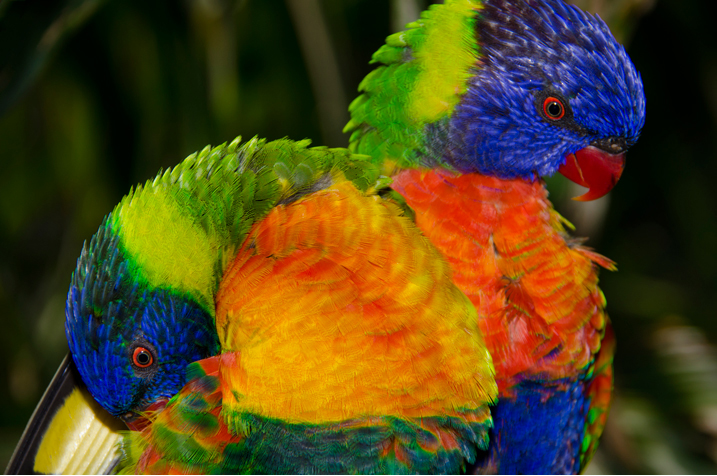
\includegraphics[width=\textwidth]{sample}

\section{GUI Section}

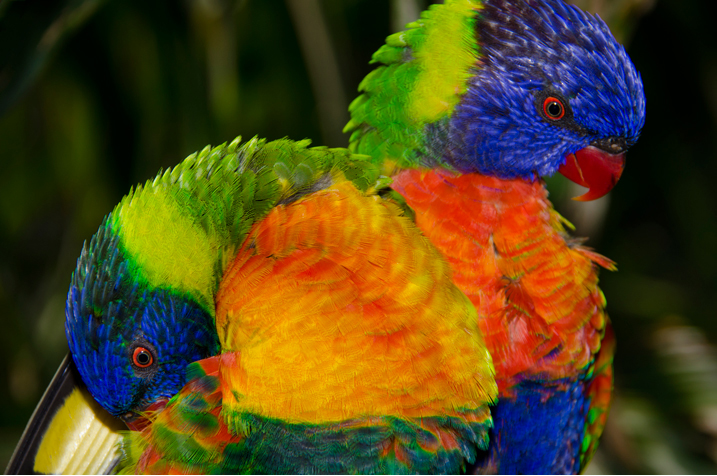
\includegraphics[trim={0 10cm 0 0},clip,width=\textwidth]{sample}
% trim={<left> <lower> <right> <upper>}

For example, show only the top of the original image for reference. asdf asdf asdf
asdf asdf asdf asdf asdf asdf asdf asdf.

There is this section that does this and that and has this stuff.

\section{GUI Section}
There will probably be a few GUI sections to elaborate on

\chapter{Another Module Name}

% picture(s) of overall gui
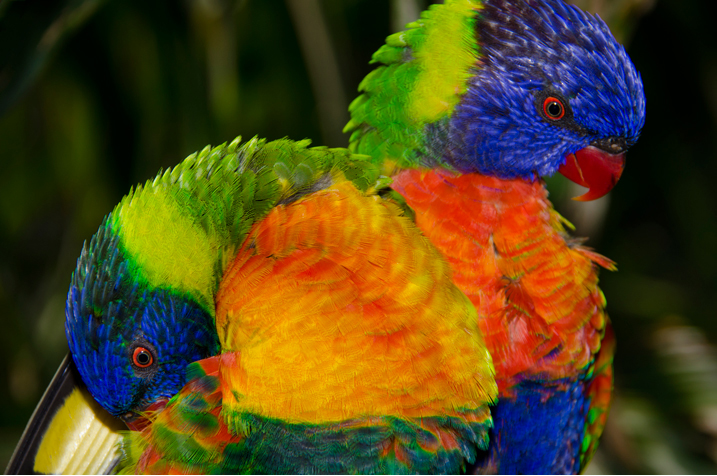
\includegraphics[width=\textwidth]{sample}

\section{GUI Section}

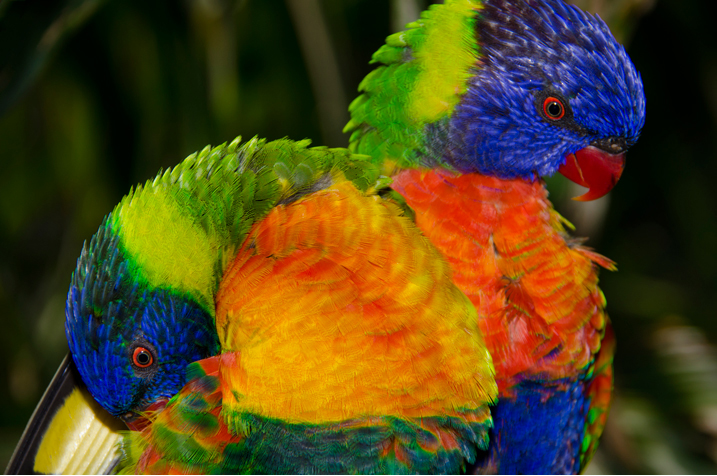
\includegraphics[trim={0 10cm 0 0},clip,width=\textwidth]{sample}
% trim={<left> <lower> <right> <upper>}

For example, show only the top of the original image for reference. asdf asdf asdf
asdf asdf asdf asdf asdf asdf asdf asdf.

There is this section that does this and that and has this stuff.

\section{GUI Section}
There will probably be a few GUI sections to elaborate on

\end{document}
